\documentclass[12pt]{article}

%%%%%%%%%%%%%%%% Commands for including graphics %%%%%%%%%%%%%%%%%%%
\usepackage{graphicx}
\DeclareGraphicsExtensions{.ps,.eps,.pcx}
%%%%%%%%%%%%%%%%%%%%%%%%%  End of these commands %%%%%%%%%%%%%%%%%
\usepackage{amsmath}
\usepackage{amssymb}
\usepackage{latexsym}
\usepackage{eucal}
\usepackage{color}
\usepackage{multirow}
\usepackage{enumitem}
\usepackage{textcomp}
\setlist{nolistsep}

\usepackage{algorithm}
\usepackage{setspace} % spacing in the algorithm
\usepackage{listings} % code Darstellung

\lstset{ 			  % code style
	backgroundcolor=\color{white},
	keepspaces=true,
	numbers=left,						% where to put the line-numbers
	numberstyle=\tiny\color{black},
	stepnumber=1,						% the step between two line-numbers
	captionpos=b,						% sets the caption-position to bottom
	tabsize=2,  						% sets default tabsize to 2 spaces
	showstringspaces=false,				% underline spaces within strings or not
	columns=flexible,
	%breaklines=true					% enter is breakline
	basicstyle={\small\ttfamily},		% the size of the fonts that are used 
	keywordstyle=\color{blue},
	commentstyle=\color{mygreen},
	stringstyle=\color{red},
	escapeinside={\%*}{*)},
	morekeywords={*,...}
}
\definecolor{mygreen}{rgb}{0,0.6,0}
\textwidth16cm


\textheight23cm

\oddsidemargin0.25cm

\evensidemargin0.25cm

\parindent0cm
\parskip2ex plus0.5ex minus0.5ex
\renewcommand{\baselinestretch}{1.37}
\unitlength1.0cm \headheight0cm \topskip0cm \headsep-1cm

\newcommand{\cov}{\mbox{cov\,}}
\newcommand{\var}{\mbox{var\,}}
\newcommand{\bbo}{\mbox{1}\hspace{-3pt}\mbox{I}}
\renewcommand{\Re}{\mbox{I}\hspace{-2pt}\mbox{R}}

\newtheorem{definition}{Definition}
\newtheorem{theorem}{Theorem}
\newtheorem{corollary}{Corollary}
\newtheorem{proposition}{Proposition}
\newtheorem{lemma}{Lemma}
\newtheorem{remark}{Remark}
\newtheorem{example}{Example}

\newcommand{\keyword}[1]{\textbf{#1}}
\newcommand{\tabhead}[1]{\textbf{#1}}
\newcommand{\code}[1]{\texttt{#1}}
\newcommand{\file}[1]{\texttt{\bfseries#1}}
\newcommand{\option}[1]{\texttt{\itshape#1}}
\newcommand{\acknowledgement}[1]{{%
		\let\thempfn\relax% Remove footnote number printing mechanism
		\footnotetext[0]{\emph{#1}}% Print footnote text
}}

%---------------------------------------------------------------------------------------
%	BIBLIOGRAPHY SETTINGS
%---------------------------------------------------------------------------------------

\usepackage[backend=bibtex, firstinits = true, maxcitenames = 2, style = authoryear, natbib = true]{biblatex} % Use the bibtex backend with the authoryear citation style (which resembles APA)

\addbibresource{BIB.bib} % The filename of the bibliography

\usepackage[autostyle=true]{csquotes} % Required to generate language-dependent quotes in the bibliography

%---------------------------------------------------------------------------------------


\begin{document}


\title{An extended exponential SEMIFAR model with application in R}
\author{Sebastian Letmathe, Jan Beran and Yuanhua Feng\\ Faculty of Business Administration and Economics, Paderborn University}
\maketitle
%\doublespacing


%\centerline{\large $^3$Swiss Federal Research Institute WSL}







\begin{abstract}
\noindent 
The paper at hand provides a detailed description of the \textit{esemifar} R-package, which is an extension of the already published \textit{smoots} package, enabling the data-driven local-polynomial smoothing of time series with long-memory. In this regard a simple data-driven algorithm is proposed based on the well-known iterative plug in algorithm for SEMIFAR (semiparametric fractional autoregressive) models. Two new functions for data-driven estimation of the trend and its derivatives under the presence of long-memory are introduced. \textit{esemifar} is applied to various environmental and financial time series with long memory, e.g. mean monthly Northern Hemisphere changes, daily observations of the air quality index of London (Britain), quarterly G7-GDP and daily trading volume of the S\&P500. It is worth mentioning that this package can be applied to any suitable time series with long memory.

  
%

\vspace{.3cm}

\noindent{\it Keywords:} long-memory, data-driven smoothing, ESEMIFAR, estimation of derivatives, \textit{esemifar} package


\vspace{.3cm}

\noindent{\it JEL Codes:} C14, C51
\end{abstract}

\acknowledgement{This paper was supported by the German DFG Project FE 1500/2-1.}
\newpage

\vspace{.5cm}

%\thispagestyle{empty}

\section{Introduction}
This paper introduces a new R-package coined \textit{esemifar} designed to supplement the already published \textit{smoots} package (smoothing time series, version 1.1.1, Feng, Schulz and Letmathe, 2021). The latter considers data-driven local polynomial smoothing of trend-stationary time series with short-range dependence. However, the literature suggests that many time series, for instance squared returns, trade durations, temperature and air pollution data, exhibit long memory (see e.g. \cite{ding1993long}, \cite{ding1996modeling}, \cite{andersen1997intraday}, \cite{andersen1999forecasting}, \cite{baillie2002modeling}, \cite{cotter2005uncovering}, \cite{beran2015modelling}, \cite{beran2017statistics} and \cite{gil2020long} among others).  
  
Against this background the \textit{esemifar} package is developed enabling the data-driven trend estimation under long memory. Analogously to \textit{smoots} the estimation of the trend and its first and second derivative is carried out by means of a data-driven IPI (iterative plug-in \cite{gasser1991flexible}) method based on the IPI for SEMIFAR (semiparametric fractional autoregressive, \cite{beran2002semifar}) models introduced by \citet{beran2002iterative}. The SEMIFAR and its exponential version the ESEMIFAR model \citep{beran2015modelling}, which is applicable to non-negative time series following a semiparametric multiplicative model form, are designed for simultaneous modelling of stochastic trends, deterministic trends and stationary short- and long-memory components in a time series.

The theoretical background of the \textit{esemifar} package and its implementation in R are briefly exemplified. For further details on the theoretical properties of the (E)SEMIFAR model and the corresponding IPI-algorithm we refer the reader to \citet{beran1999semifar}, \citet{beran2002semifar}, \citet{beran2002iterative}, \citet{beran2002local}, \citet{beran2015modelling}, \citet{beran2016long} and references therein. The main objective of this paper is the introduction of the \textit{esemifar} package and the illustration of its usefulness in particular for non-stationary time series exhibiting a long-memory dependence structure. That is achieved by employing our package to different environmental as well as financial time series. We partly exploit data that was already used by Feng et al. (forthcoming), namely monthly Northern Hemisphere temperature changes, as the authors already indicated that this data might exhibit long range dependence. In addition to that \textit{esemifar} is applied to daily observations of the (composite) air quality index of London (Britain). And, analogously to Feng et al. (forthcoming) \textit{esemifar} is used in the context of a semiparametric log-local-linear growth model for analysing quarterly G7 GDP data. Moreover, it was first indicated by \citet{beran2015modelling} that the (type 1) Log-ACD model introduced by \citet{bauwens2000logarithmic}, \citet{bauwens2008moments} and \citet{karanasos2008statistical} can be represented as an EFARIMA model. Subsequently, it was shown by \citet{feng2015forecasting} that the EFARIMA and ESEMIFAR can be redefined as a FI-Log-ACD and a Semi-FI-Log-ACD, respectively. We illustrate the use of \textit{esemifar} in regards to the Semi-FI-Log-ACD by modelling log-transformed trading volume of the S\&P500.

The paper is organised as follows. In Section 2 the definitions of the (E)FARIMA and (E)SEMIFAR are given and the methodological background as well as the IPI-algorithm incorporated in \textit{esemifar} are elaborated. The implementation in R is exemplified in Section 3. The application of our proposal to environmental data is illustrated in Section 4. The use of \textit{esemifar} within the scope of the Semi-FI-Log-ACD is investigated in Section 5. In Section 6 final remarks are given.

\section{Smoothing long memory time series}
In the sequel, the definitions of the well known (E)FARIMA and (E)SEMIFAR models (see \cite{beran1999semifar}, \cite{beran2002semifar} and \cite{beran2015modelling}) and local polynomial smoothing for long memory time series are briefly exemplified. Moreover, a modified version of the 
IPI for SEMIFAR models (see \cite{beran2002iterative}) is proposed.

\subsection{The (E)FARIMA and (E)SEMIFAR}
A well-established model for  analysing financial time series data is the multiplicative error model (MEM) (\cite{engle2002dynamic})  which is given by 
\begin{equation}
\label{MEM}
X_t=s \lambda_t \eta_t,
\end{equation}
where the scale parameter is denoted by $s >0$, $\lambda_t >0$ denotes the conditional mean of $X^*=X_t/s$, and $\eta_t$ are i.i.d. random variables with $\epsilon_t = \ln(\eta_t)$ such that $E(\epsilon_t) = 0$ and $\sigma^2_\epsilon = \var(\epsilon_t)$ . Following Feng and Zhou (2015) we can rewrite \eqref{MEM} as a semiparametric MEM given by
\begin{equation}
\label{SMEM}
X_t=s(\tau_t)\lambda_t \eta_t,
\end{equation}   
where $\tau_t=t/n$ denotes the rescaled time and where the scale parameter $s$ in \eqref{MEM} is replaced with a nonparametric scale function denoted by $s(\tau_t)$. 
By taking the logs of \eqref{SMEM} we have
\begin{equation}
\label{SEMIFAR}
Y_t=g(\tau_t) + Z_t,
\end{equation}
where $Y_t=\ln(X_t)$, $g(\tau_t)=\ln[s(\tau_t)]$, $Z_t=\ln(\lambda_t) + \epsilon_t$. % and $\epsilon_t=\ln(\eta_t)$.
Following \citet{beran2002semifar} we assume that $Z_t$ follows a zero mean FARIMA ($p, d, q$) process, which is given by
\begin{equation}
\label{FARIMA}
(1-B)^d\phi(B)Z_t =\psi(B)\epsilon_t,
\end{equation}
where $d \in (0,0.5)$ is the long-memory parameter, $B$ is the backshift operator, $\phi(z)=1-\sum_{i=1}^{p}\phi_iz^i$ and  $\psi(z)=1+\sum_{i=1}^{q}\psi_iz^i$ are AR- and MA-polynomials with all roots outside the unit circle. The long-memory parameter $d$ was introduced by \citet{granger1980introduction} and \citet{hosking1981fractional} and is defined by 
\begin{equation}
	\label{d}
	(1-B)^{d} = \sum_{k=0}^{\infty} b_k(d) B^k, 
\end{equation} 
where $b_k(d) = (-1)^{k}{d\choose k}  = (-1)^{k} \frac{\Gamma(d+1)}{\Gamma(k+1)\Gamma(d-k+1)}$ and $\Gamma(\cdot)$ denotes the Gamma function. Equation \eqref{FARIMA} defines a stationary and invertible FARIMA process with $E(\epsilon_t)=0$ and $var(\epsilon_t)=\sigma^2_{\epsilon}$. Model \eqref{SEMIFAR} is equivalent to a SEMIFAR process (\cite{beran2002semifar}) with no integer differencing ($m=0$) and an additional MA-part.
Subsequently, model \eqref{SMEM} is an ESEMIFAR introduced by \citet{beran2015modelling}.
%However, the authors assumed that $X^*_t$ is log-normally distributed whereas in this paper we relax this assumption and suppose that $X_t^*$ satisfies condition \textbf{A1} of \citet{feng2020fractionally}.
%Please note that $X^*_t = \exp(Z_t)$.

\subsection{Local polynomial regression for long memory time series}
In the following local polynomial estimation of the scale function $g^{(\nu)}$, the $\nu$-th derivative of $g$, is exemplified briefly (see e.g. \cite{beran2002iterative}, \cite{beran2002local}, \cite{beran2002semifar}, and \cite{beran2013limit}). Under the assumption that $g$ is at least ($l+1$)-times differentiable at a point $t_0$, $g(\tau_t)$ can be approximated by a local polynomial of order $l$ for $\tau_t$ in a neighbourhood of $\tau_0$. Following \citet{gasser1979kernel}, the weight function is determined to be a second order kernel with compact support $[-1,1]$ having the polynomial form $K(u)=\sum_{i=0}^{r}a_i u^{2i}$, for $(|u|\leq1)$,where $K(u)=0$ if $|u|>1$ and $a_i$ are such that $\int_{-1}^{1}K(u)du=1$ holds.  Here, $r \in \{0,1,2,3\}$ denotes the kernel used for estimating $g^{(\nu)}$, corresponding to the uniform, epanechnikov, bisquare and triweight kernel, respectively.
$\hat{g}^{(\nu)}$ ($\nu\leq l$) can now be obtained by solving the locally weighted least squares problem
\begin{equation}
\label{LP}
Q=\sum_{i=1}^{t}\Bigg[Y_t-\sum_{j=0}^{l}b_j(\tau_i-\tau_0)^j\Bigg]^2 K\Big(\frac{\tau_i-\tau_0}{h}\Big),	
\end{equation}
where $h$ denotes the bandwidth and $K[(\tau_i-\tau_0)/h]$ are the weights ensuring that only observations in the neighbourhood of $\tau_0$ are used. Consider the case where $l-\nu$ is odd. Define $m=l+1$, then we have $m \geq \nu + 2$ and $m-\nu$ is even. A point $\tau$ is said to be in the interior for each $\tau_t\in [h,1-h]$, at the left boundary if $\tau_t\in [0,h)]$ and at the right boundary if $\tau_t\in (1-h,1]$. Following \citet{beran2002local} a common definition for an interior point is $\tau=ch$ with $c=1$ and for a boundary point we have $c \in [0,1)$.   
Asymptotic expressions for the bias, variance and mean integrated squared error (MISE) are presented in Theorem 1 and 2 by \citet{beran2002local}. The asymptotic mean integrated squared error (AMISE) is given by
\begin{equation}
	\label{AMISE}
	\text{AMISE}(h) = h^{2(m-\nu)} \frac{I[g^{(m)}]\beta^2}{m!} + \frac{(nh)^{2d-1}V(1)}{h^{2\nu}},
\end{equation}
where $I[g^{(m)}] = \int_{c_b}^{d_b}[g^{m}(\tau)]^2d\tau$ with $0 \leq c_b < d_b \leq 1$ in order to reduce the so-called boundary effect. Moreover, $\beta = \int_{-1}^{1}u^mK(u)du$ and for $d > 0 $ we have $V(1)=2c_f \Gamma(1-2d)\sin (\pi d) \int_{-1}^{1} \int_{-1}^{1} K(x)K(y)|x-y|^{2d-1}dxdy$. For $d = 0$, $V$ reduces to $V(1)=2\pi c_f \int_{-1}^{1}K^2(x)dx$. $c_f$ stands for the spectral density of the ARMA part of \eqref{FARIMA} at frequency zero and is given by 
\begin{equation}
	c_f = f(0) = \frac{\sigma^2_\epsilon}{2\pi} \frac{(1 + \psi_1+\dots+\psi_q)^2}{(1-\phi_1-\dots-\phi_p)^2}.
\end{equation}
 The asymptotically optimal bandwidth, denoted by $h_A$, that minimizes the AMISE is given by
\begin{equation}
	\label{ha1}
h_A=Cn^{(2d-1)/(2m+1-2d)},
\end{equation}
with 
\begin{equation}
\label{ha2}
C=\Bigg(\frac{[m!]^2}{2(m-\nu)} \frac{(2\nu+1-2d)}{\beta^2}\frac{(d_b - c_b)V(1)}{I[g^{(m)}]}\Bigg)^{1/(2m+1-2d)}.
\end{equation} 
In order to obtain a selected bandwidth the unknown constants $I[g^{(m)}]$, $d$ and $V$ in \eqref{ha1} have to be replaced with consistent estimators. Please note, that the estimation of $V$ relates to that of $c_f$. $I[g^{(m)}]$ is estimated by means of local polynomial regression and numerical integration. The remaining two quantities $d$ and $V$ can be obtained via maximum likelihood. Inserting those estimates into \eqref{ha1} yields a plug-in estimator for the bandwidth, which minimises the MISE.

Based on these results \citet{beran2002iterative} proposed two iterative plug-in algorithms for automatic bandwidth selection, namely Algorithm \textbf{A} and \textbf{B}. In this paper we only consider a strongly adapted version of Algorithm \textbf{B} which is presented in the following.
\subsection{The IPI-algorithm for estimating $g$}

We introduce a modified IPI-procedure for SEMIFAR models by translating and adapting the main features of the IPI for SEMIFAR models introduced by \citet{beran2002iterative} from the programming language S to R. The algorithm processes as follows:

\begin{itemize}
	\item[\textbf{i)}] In the first iteration start with an initial bandwidth $h_0$ set beforehand and select $p$ and $q$ denoting the AR- and MA-order, respectively. 

	\item [\textbf{ii)}] Estimate $g$ from $Y_t$ employing $h_{j-1}$ and calculate the residuals $\tilde{Z}_t = Y_t - \hat{g}(\tau_t)$. Estimate $d$ and $V$ by fitting a FARIMA (with predefined AR- and MA-order in Step i) to  $\hat{Z}_t$.
			
	\item [\textbf{iii)}] Set $h_{d,j}=(h_{j-1})^\alpha$, where $\alpha$ denotes an 
		inflation factor. Estimate $I[g^{(m)}]$ via a local polynomial of order $l^* = l + 2$ and with $h_d,j$. Now, we obtain $h_{j-1}$ by 
		\begin{equation}
			h_j=\Bigg(\frac{[m!]^2}{2m} \frac{(1-2\hat{d})}{\beta^2}\frac{(d_b - c_b)\hat{V}(1)}{I[\hat{g}^{(m)}]}\Bigg)^{1/(2m+1-2\hat{d})}\cdot n^{(2\hat{d}-1)/(2m+1-2\hat{d})}.
		\end{equation}
	
	\item [\textbf{iv)}] Repeat steps ii) and iii) until convergence or a given number of iterations has been reached and set $\hat{h}_{opt} = h_j$.	
\end{itemize}
We propose to set the initial bandwidths to $h_0 = 0.1$ for $l = 1$ and $h_0 = 0.2$ for $l = 3$. Moreover, for $p = 3$ it is recommended to employ $c_b = 1 - d_b$ such that only 90\% of all observations are used for estimating an interior point in order to reduce the boundary effect. For $l = 1$ all observations are used and hence $c_b = 1 - d_b = 0$. The bandwidth $h_{d.j}$ used for estimating $g^{(m)}$ is enlarged by means of an exponential inflation factor denoted by $\alpha$. We have $\alpha = \alpha_{\text{opt}} = (2m + 1 - 2d) / (2m + 3 - 2d)$, $\alpha = \alpha_{\text{nai}} = (2m + 1 - 2d) / (2m + 5 - 2d)$ and $\alpha = \alpha_{var} = \frac{1}{2}$. Using $\alpha_{\text{opt}}$ results in bandwidth $h_{d,j}$ that minimizes the MSE of $\hat{I}[g^{(m)}]$ and consequently the rate of convergence of $\hat{h}_j$ is optimal. Whereas for $\alpha_{\text{nai}}$ the optimal rate of convergence is achieved for $\hat{m}^{(m)}$ and $\alpha_{\text{var}}$ ensures a stable selection of the bandwidth. Moreover, we have $\alpha_{\text{var}} > \alpha_{\text{nai}} > \alpha_{\text{opt}}$ and $\alpha_{\text{nai}} \rightarrow \alpha_{\text{var}}$ as $d \rightarrow 0.5$. The choice of $\alpha$ depends on the underlying data, which is to be analysed. For a more detailed insight on inflation methods we refer the reader to \citet{beran2002iterative}.   

%Please note that the results presented in \citet{beran1999semifar}, \citet{beran2001volatility}, \citet{beran2002iterative}, \citet{beran2002local}, \citet{beran2002semifar} and \citet{beran2016long} remain valid for the IPI for SEMIFARIMA models.    

\subsection{Data-driven estimation of g\textquotesingle{} and g\textquotesingle \textquotesingle}
The modified IPI for SEMIFAR models can also be applied to bandwidth selection for estimating $g^{(\nu)}$ with $\nu > 0$. In this paper, only the cases for $\nu = 1$ and $\nu = 2$ are discussed. The proposed IPI is now employed as a data-driven pilot method to obtain estimates for $d$, $c_f$ and $h_{\nu, 0}$ with order $l_d$, say. Estimation of $g^{(\nu)}$ is then carried out with $l = \nu + 1$ and $m = \nu + 2$. As previously, $g^{(m)}$, which is required for calculating $I[g^{(m)}]$ is estimated with order $l^* = l + 2$. The following two-stage procedure is proposed.
\begin{itemize}
	\item[\textbf{i)}] In the first stage $\hat{d}$, $\hat{c}_f$, and $\hat{h}_{\text{opt}}$ are obtained by means of the main IPI-algorithm for estimating $g$ with order $l_d = 1$ or $l_d = 3$.
	
	\item[\textbf{ii)}] Set $h_{\nu,0} = \hat{h}_{\text{opt}}$. Carry out an IPI-procedure as proposed above with fixed $\hat{c}_f$ and $\hat{d}$ in order to select a bandwidth for estimating $g^{(\nu)}$. Please note that \eqref{ha1} should be used. 
\end{itemize}
Explicit formulas of the equivalent kernels for estimating $g^{(\nu)}$ at an interior point $\tau_t$ can be found in \citet{muller1988longitudinal}. The corresponding inflation factors are defined as previously and are determined by $m$ and $d$.

\section{Implementation in R}
Based on the algorithms introduced in the previous section a R-package is developed, which is an extension of the already published \textit{smoots} package. Hence, this package will be coined \textit{esemifar}. The main functions are called \textit{tsmoothlm} and \textit{dsmoothlm} for estimating the trend and its derivatives, respectively, under presence of long-memory errors. Local polynomial estimation of  $g^{(\nu)}$ and kernel smoothing of $g$ are carried out by means of the functions \textit{gsmooth} and \textit{knsmooth}, which are implemented in the \textit{smoots} package (see Feng et al., forthcoming).

In the following the function \textit{tsmoothlm} is explained in more detail. The first argument $y$ denotes the input time series. The second and third argument (\textit{pmin} and \textit{pmax}) are the minimum and maximum AR-order of the stochastic part $Z_t$ in \eqref{SEMIFAR}, respectively. Accordingly, the fourth and fifth argument (\textit{qmin} and \textit{qmax}) stand for the the minimum and maximum MA-order of $Z_t$. All four arguments can take the value 0, 1, 2, 3, 4 or 5 while $p_{\text{min}} \leq  p_{\text{max}}$ and $q_{\text{min}} \leq  q_{\text{max}}$. The optimal order is determined via BIC. The default setting is $p_{\text{min}} = q_{\text{min}} = p_{\text{max}} = q_{\text{max}} = 0$. The order of the polynomial for trend estimation is set via the argument $p$ and the user can choose between 1 and 3, where $p = 1$ is the predefined option. The argument \textit{mu} controls for the smoothness of the weight function. We have $\mu \in \{0,1,2,3\}$, with $\mu = 1$ for the Epanechnikov kernel as default. Furthermore, the inflation factor $\alpha$ can be selected by the argument \textit{InfR} with three different options, i.e. \textit{``Opt"}, \textit{``Nai"} and \textit{``Var"}, which corresponds to $\alpha_{\text{opt}} = (2m + 1 - 2d) / (2m + 3 - 2d)$, $\alpha_{\text{nai}} = (2m + 1 - 2d) / (2m + 5 - 2d)$ and $\alpha_{var} = \frac{1}{2}$, respectively. The default setting for \textit{InfR} is \textit{``Opt"}.
Moreover, the starting bandwidth $h_0$ can be set beforehand by the argument \textit{bStart} with default $h_0 = 0.15$. However, the choice of \textit{bStart} should not affect the finally selected bandwidth if the IPI converges. Argument \textit{bb} controls for boundary bandwidth. The default is $bb = 1$ meaning that the k-nearest neighbour method is applied, which results in a total bandwidth of $2\hat{h}$ at each observation point $\tau_t$. For $\textit{bb} = 0$ however, the total bandwidth is shortened at boundary points. By the argument \textit{cb}, which is set to $\textit{cb} = 0.05$ per default, the percentage of observations omitted for calculating $I[g^{(m)}] = \int_{c_b}^{1-d_b}[g^{m}(\tau)]^2d\tau$ in \eqref{ha1} can be controlled. Additionally, the smoothing method with $\hat{h}_{\text{opt}}$ can be selected via the argument \textit{method}. The user may choose between local polynomial regression (``\textit{lpr}") and kernel regression (``\textit{kr}"). However, originally kernel regression has been only incorporated in the \textit{smoots} package as a benchmark to local polynomial regression.

For estimating $g^{(\nu)}$ the function \textit{dsmoothlm} is applied. Please recall that here \textit{tsmoothlm} is employed as a pilot method with minimum and maximum AR- and MA-order \textit{pmin}, \textit{pmax}, \textit{qmin} as well as \textit{qmax}, a local polynomial estimator of order \textit{pp}, the inflation rate \textit{InfR.p}, the kernel \textit{mu.p} and a starting bandwidth \textit{bStart.p} in order to obtain initial estimates for $\hat{d}$, $\hat{c_f}$ and $\hat{h}_{\nu,0}$ (see section 3.2). The options and default settings for these arguments are the same as for \textit{tsmoothlm}. In addition to that, the order of the derivative to be estimated is set via the argument \textit{d} and can take the value 1 or 2 for the first and second derivative, respectively. Moreover, the argument \textit{mu} controls the kernel used for bandwidth selection after the pilot stage. Please note that S3 methods (\textit{print} and \textit{plot}) along the lines of the \textit{smoots} package can be employed to the estimation results of the functions above. The output objects of \textit{tsmoothlm} and \textit{dsmoothlm} are basically lists containing input parameters and estimation results. Further detailed information on the functions are to be published in the users guideline of the \textit{esemifar} package.       


\section{Application of the SEMIFAR and ESEMIFAR}
In this section the SEMIFAR and ESEMIFAR are applied to four real data examples: \textit{tempNH} (mean monthly temperature changes), \textit{aqiLDN} (daily air quality index) and \textit{gdpG7} (G7 GDP). An old version of the \textit{tempNH} data set has already been subject to an application example in \citet{feng2007asymptotic}, where the author employed the original version of the IPI for SEMIFAR models. An updated version of $\textit{tempNH}$ is implemented in the \textit{smoots} package, which was recently published on the \textit{CRAN} network, and the remaining two data sets will be available in \textit{esemifar}. 

\subsection{Application to environmental data}
The SEMIFARIMA defined by \eqref{SEMIFAR} is applied to the time series of mean monthly Northern Hemisphere temperature changes (NHTM) from 1880 to 2018. The data is available at the website of the National Aeronautics and Space Administration (NASA). Bandwidth selection is carried out by means of the IPI for SEMIFARIMA models introduced in section 3. For model- and bandwidth selection the \textit{tsmoothlm} function is applied, with $\textit{p} = 1$, $\textit{pmin} = \textit{qmin} = 0$, $\textit{pmax} = \textit{qmax} = 3$ and $\textit{InfR} = \textit{``Opt"}$. The remaining arguments are set on their default. 

In Figure 1a) the fitted trend together with the observations is illustrated. The optimal bandwidth is $\hat{h}_{\text{opt}} = 0.165$ and a FARIMA ($0, \hat{d}, 0$) has been selected following the BIC with $\hat{d} = 0.405$ implying strong long-range dependence in the temperature data. Apparently, the SEMIFARIMA captures the trend quite well. A clear upward trend can be observed approximately after 1970, which could be interpreted as an indicator for global warming. The trend-adjusted residuals are shown in Figure 1b) and first and second derivative are depicted in Figures 1c) and 1d), respectively. Please note that for the estimation of derivatives the dependence structure has been estimated by pilot smoothing with order $\textit{pp} = 3$. The derivatives match the features of the trend shown in Figure 1a) and provide further information about global temperature changes. For instance the slope of the first derivative indicates how strong the trend is increasing or decreasing. The intersections of the second derivative with the x-axis indicate a shift in the slope of $\hat{g}$. 
 
\begin{figure}[!h]
		\includegraphics[trim = {0cm 0mm 0mm 0mm}, width = \textwidth]{Abb/NHtemp.pdf}
		\caption{Estimated trend, residuals and the trend`s derivatives for the NHTM series}
\end{figure}

Moreover, the ESEMIFAR defined by \eqref{SMEM} is applied to daily observations of the (composite) air quality index (AQI) of London from 2014 to 2020. The composite AQI is simply the maximum of all individual AQI of particulate matter less than 2.5 and 10 microns (PM25 and PM10), Ozone (O3) , Nitrogen Dioxide (NO2), Sulfur Dioxide (SO2) and Carbon monoxide (CO). The data can be obtained from the European Environment Agency. An ESEMIFAR is fitted to the log-transformed air quality index series, again, by means of the \textit{tsmoothlm} function. Here, the inflation rate is set to $\textit{InfR} = \textit{``Var"}$ due to the large variation in the data and again a local linear smoother is employed, i.e. $p = 1$. Moreover, $\textit{pmin} = \textit{qmin} = 0$, $\textit{pmax} = \textit{qmax} = 1$ and all other arguments are set on their default.
 

Figure 2a) depicts the log-transformed air quality index series together with the estimated trend. The optimal bandwidth amounts to $\hat{h}_{opt} = 0.242$ and a FARIMA ($1, \hat{d}, 0$) is selected by the BIC with $\hat{\phi}_1 = 0.544$ and $\hat{d} = 0.103$. Trend adjusted residuals, first and second derivative are depicted in Figures 2b), 2c) and 2d), respectively. Our results indicate that the ESEMIFAR fits the data very well. We observe a slight downward trend of air pollution beginning in the middle of 2017 and continuing to the end of 2020. However, a deeper interpretation of our results in regard of an environmental context is beyond the scope of this paper.    

 

\begin{figure}[!h]
	\label{aqi}
	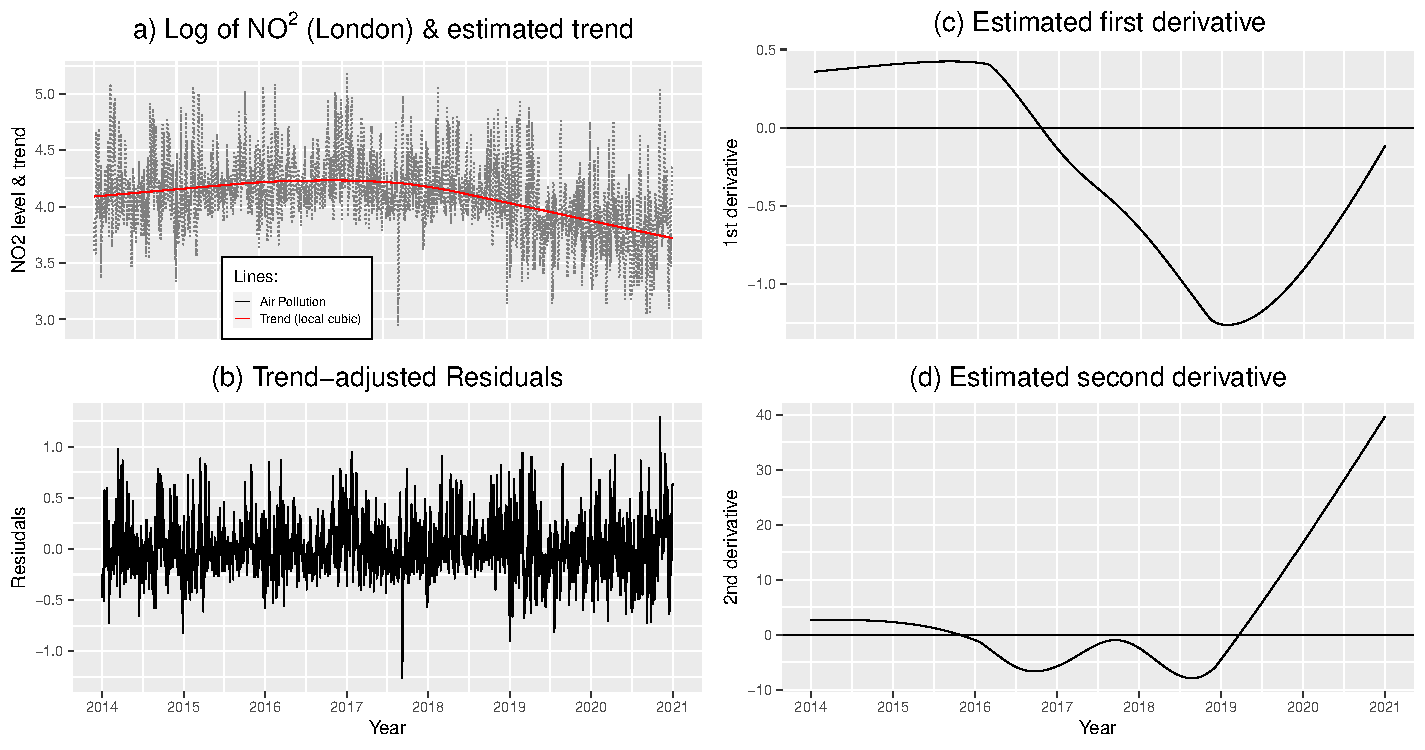
\includegraphics[trim = {0cm 0mm 0mm 0mm}, width = \textwidth]{Abb/London_AirQuality_AQI_linear.pdf}
	\caption{Estimated trend, residuals and the trend`s derivatives for the AQI series}
\end{figure}

\subsection{Application to GDP data}
A model which is commonly used in the field of macroeconomic research is the well-known log-linear growth model. Feng et al. (2020) have achieved a semiparametric local-linear extensions of this model by applying a Semi-ARMA to log-transformed GDP series. We follow this approach and additionally incorporate long memory by assuming that the log-transformed quarterly G7-GDP series from 1961 to 2019 follows a SEMI-FARIMA defined by \eqref{SEMIFAR} and \eqref{FARIMA}. The data was obtained from the Organisation for Economic Co-operation and Development (OECD). For this purpose the \textit{tsmoothlm} function is employed, with $\textit{p} = 1$, $\textit{pmin} = \textit{qmin} = \textit{pmax} = \textit{qmax} = 1$ and $\textit{InfR} = \textit{``Opt"}$. The remaining arguments are set on their default. We obtained an optimal bandwidth of 0.112 and a FARIMA ($1,\hat{d},1$) with $\hat{d} = 0.252$, and $\hat{\phi}_1 = 0.858$ and $\hat{\psi}_1 = 0.192$ is fitted to the residuals.

As a benchmark a kernel regression is carried out using the same bandwidth. Estimated trends together with log-gdp series are shown in Figure 2(a). At the interior both estimators are approximately equal. However, we can see that the kernel estimator clearly shows poor estimation quality at the boundaries which indicates that the local-linear estimator is to be preferred. The trend-adjusted residuals obtained by the local-linear approach are depicted in Figure 2(b). Moreover, the corresponding derivatives are illustrated in Figures 2(c) and 2(d), which reveal further information on the course of the economy.
 
\begin{figure}[h!]
	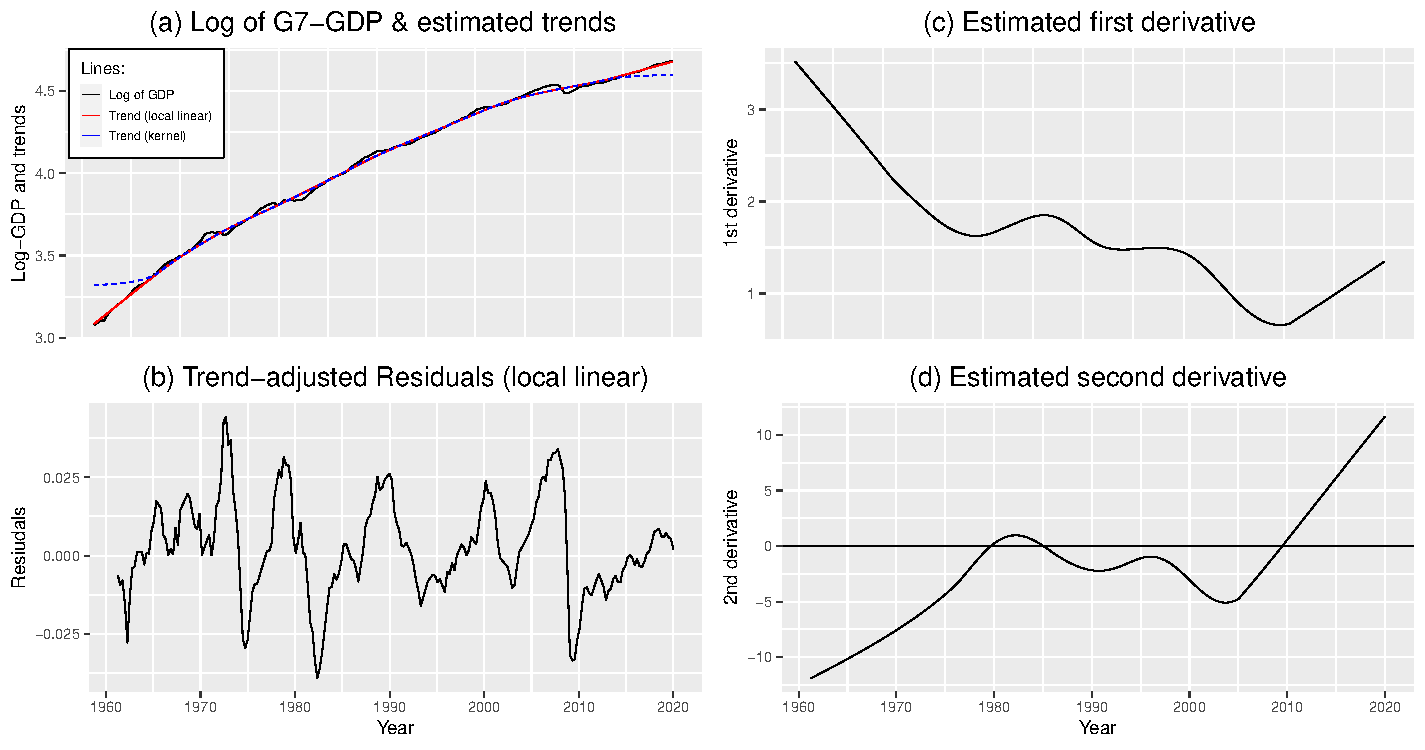
\includegraphics[trim = {0cm 0mm 0mm 0mm}, width = \textwidth]{Abb/G7gdp.pdf}
	\caption{Estimated trend, residuals and the trend`s derivatives for the G7-GDP series}
\end{figure}


\section{Application to financial data}
 Another well-known method for analysing non-negative financial time series is the autoregressive conditional duration (ACD) model introduced by \citet{engle1998autoregressive}. An extension of the ACD is the (type 1) Log-ACD$_1$ proposed by \citet{bauwens2008moments} which can considered to be a squared version of the Log-GARCH. A fractionally integrated generalization of the Log-ACD was indicated by \citet{beran2015modelling} and subsequently \citet{feng2015forecasting} proposed the FI-Log-ACD and its semiparametric extension the Semi-FI-Log-ACD. Moreover, the authors showed that the FI-Log-ACD (Semi-FI-Log-ACD) is equivalent to the EFARIMA (ESEMIFAR). Hence, the Semi-FI-Log-ACD can be estimated by the \textit{esemifar} package. For a detailed derivation of the Semi-FI-Log-ACD we refer the reader to \citet{feng2015forecasting}.

 In the following the ESEMIFAR is applied to daily trading volume of the S\&P500 from January 2000 to December 2020. The data was obtained from Yahoo finance. The original series is displayed in Figure 4a) and it can be seen that the variation in the data is clearly time dependent. Trend estimation is carried out with a local linear and cubic smoother ($p = 1$ and $p = 3$). The model order is set to  $\textit{pmin} = \textit{qmin} = \textit{pmax} = \textit{qmax} = 1$. For $p=1$ and $p=3$ the selected bandwidths are 0.085 and 0.191, respectively. In Figure 4b) the log-transformed series, the local linear and local cubic trends are shown and are indicated by the black, red and blue (dashed) lines, respectively. Both estimators deliver very satisfying results but the local cubic approach seems to slightly over-fit the data. Therefore, the conditional and total means illustrated in Figures 4c) and 4d) as well as the residuals are obtained from the local linear estimates. From the residuals of the local linear estimator we obtain a FARIMA($1, \hat{d}, 1$) model with $\hat{\phi}_1 = 0.553$, $\hat{\psi}_1 = 0.410$ and $\hat{d} = 0.319$ indicating moderately strong long-range dependence in the data. 
 
 
 \begin{figure}[h!]
 	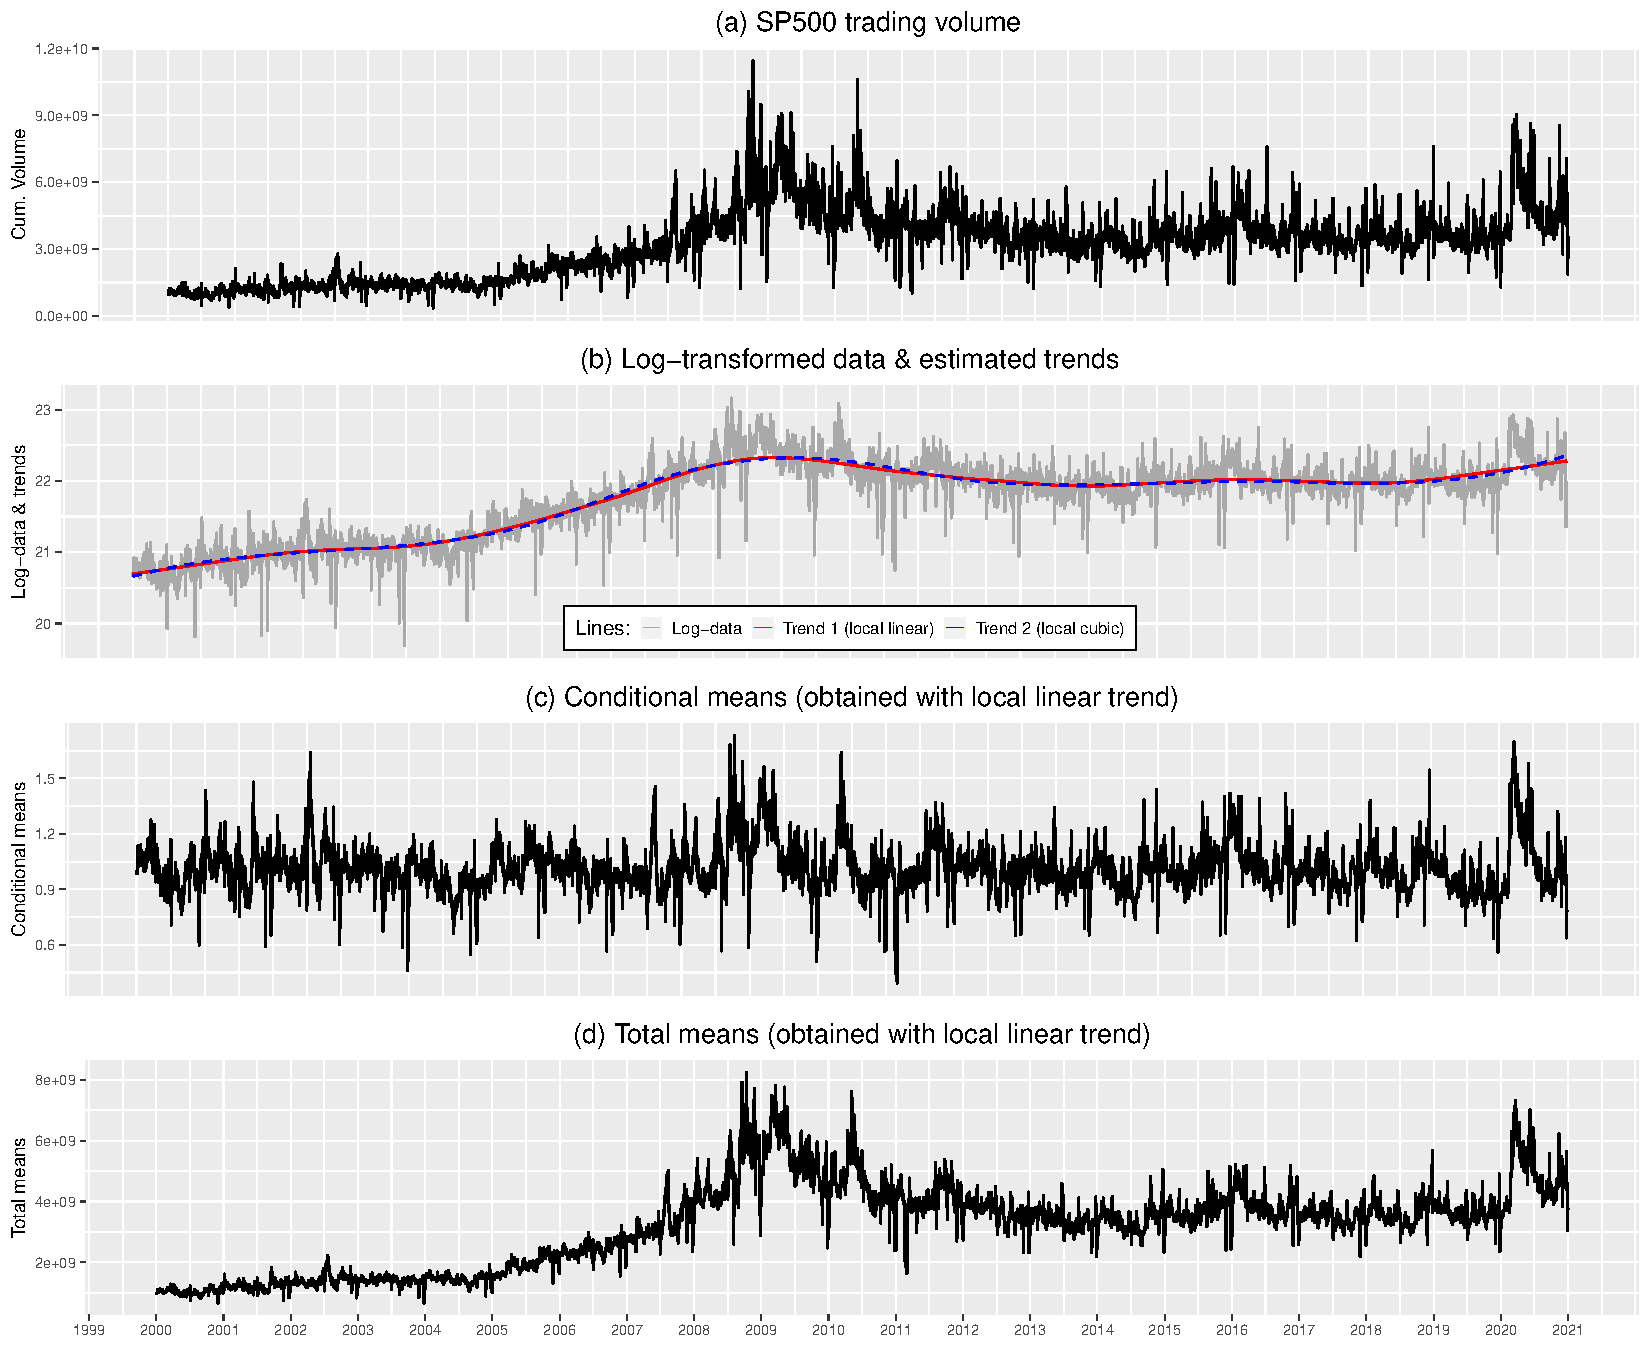
\includegraphics[trim = {0cm 0mm 0mm 0mm}, width = \textwidth]{Abb/SP500VOL.pdf}
 	\caption{Estimation results of the ESEMIFAR for the SP500 series.}
 \end{figure}


\section{Concluding remarks}
The paper at hand exemplifies the development of a supplementing R-package for the \textit{smoots} package. The main feature of this package is the semi-parametric estimation under long-memory errors, which to the best of our knowledge has not been possible before at least within the scope of R. In this regard an adapted version of the iterative plug in algorithm proposed by \citet{beran2002iterative} is introduced. Moreover, the implementation of this package is comprehensively described. The usage of two main functions is explained and illustrated by application to various non-stationary time series with long-memory. The estimation results are quite satisfactory and illustrate the wide applicability of our proposal. Further extensions of \textit{esemifar} are the implementation of a forecasting procedure and the non-parametric estimation of the stochastic part of the model by means of e.g.  a local Whittle-, GPH- or wavelet-estimator.

%\vspace*{\fill}
%\textbf{Acknowledgement:} This paper was supported by the German DFG Project FE 1500/2-1. The sources of the used data are acknowledged in the context with corresponding references. We are grateful to Ms. Shujie Li, Mr. Bastian Schäfer and Mr. Dominik Schulz at Paderborn University, Germany, for helpful discussions and suggestions.
\clearpage

\printbibliography


\clearpage
%section*{Appendix}





\end{document}
